\chapter{Auswertung}
\section{Entwicklung einer Metrik}
\begin{tabular}{|c|c|c|c|c|}
	\hline
	-- & - & 0 & + & ++ \\
	\hline
	0 & 1 & 2 & 3 & 4 \\
	\hline
\end{tabular}
Balkendiagramm mit durchschnittlicher Bewertung und Bewertung von Reem und Timo
\section{Entwicklung der Kinder}
\subsection{Jonas}
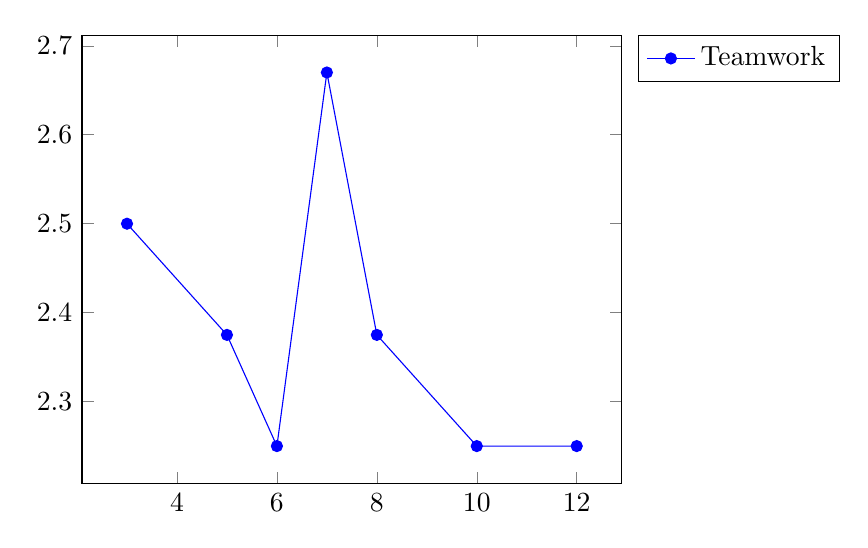
\begin{tikzpicture}
	\begin{axis}[legend pos=outer north east]
		\addplot[mark=*,blue]
		coordinates {
			(3,2.5) (5,2.375) (6,2.25) (7,2.67) (8,2.375) (10,2.25) (12,2.25)
		};
		\legend{Teamwork}
	\end{axis}
\end{tikzpicture}

\subsection{Mario}
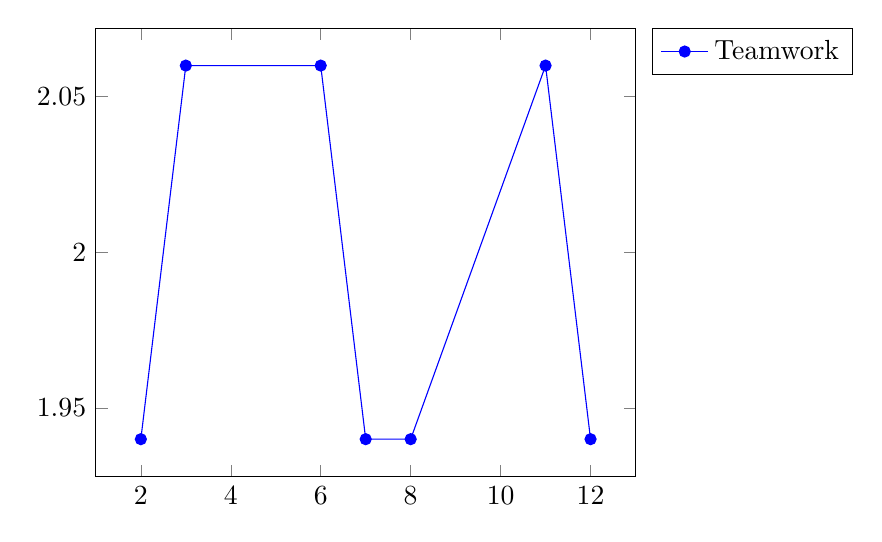
\begin{tikzpicture}
	\begin{axis}[legend pos=outer north east]
		\addplot[mark=*,blue]
		coordinates {
			(2,1.94)(3,2.06)(6,2.06)(7,1.94)(8,1.94)(11,2.06)(12,1.94)
		};
		\legend{Teamwork}
	\end{axis}
\end{tikzpicture}

\subsection{Sara}
\begin{tikzpicture}
	\begin{axis}[legend pos=outer north east]
		\addplot[mark=*,blue]
		coordinates {
			(3,.47) (5,.47) (6,.5) (7,.38) (8,0.93) (11,.88) (12,.93)
		};
		\legend{Teamwork}
	\end{axis}
\end{tikzpicture}


\subsection{Benny}
\begin{tikzpicture}
	\begin{axis}[legend pos=outer north east]
		\addplot[mark=*,blue]
		coordinates {
			(2,1.45)(3,1.31) (5,2.37) (6,2.06) (7,1.4) (8,1.33) (10,.57) (11,.5)(12,.54)
		};
		\legend{Teamwork}
	\end{axis}
\end{tikzpicture}


\subsection{Henriette}
\begin{tikzpicture}
	\begin{axis}[legend pos=outer north east]
		\addplot[mark=*,blue]
		coordinates {
			(2,2.21)(3,2)(5,2.31)(6,1.19)(7,1.75)(8,1.88)(10,1.79)(11,0.63)(12,0.63)
		};
		\legend{Teamwork}
	\end{axis}
\end{tikzpicture}

\subsection{Moritz}
\begin{tikzpicture}
	\begin{axis}[legend pos=outer north east]
		\addplot[mark=*,blue]
		coordinates {
			(2,2.43)(3,2.43)(5,1.5)(6,1.2)(10,1.33)(11,.73)(12,.53)
		};
		\legend{Teamwork}
	\end{axis}
\end{tikzpicture}


\subsection{Lulu}
\begin{tikzpicture}
	\begin{axis}[legend pos=outer north east]
		\addplot[mark=*,blue]
		coordinates {
			(2,2.01)(3,2.43)(5,1.14)(6,1.5)(7,1)(8,.67)(10,1)(11,.43)(12,.38)
		};
		\legend{Teamwork}
	\end{axis}
\end{tikzpicture}


\subsection{Heinz}
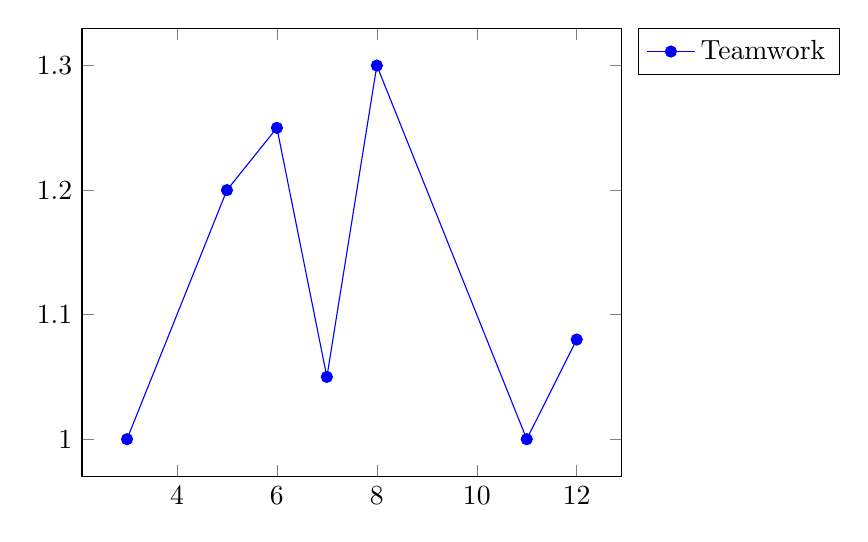
\begin{tikzpicture}
	\begin{axis}[legend pos=outer north east]
		\addplot[mark=*,blue]
		coordinates {
			(3,1)(5,1.2)(6,1.25)(7,1.05)(8,1.3)(11,1)(12,1.08)
		};
		\legend{Teamwork}
	\end{axis}
\end{tikzpicture}

\section{Persönlichkeitstypen und Entwicklung}
Liniendiagramm mit Termin auf X-Achse und Durchschnittswert der Persönlichkeitstypen auf Y-Achse


\subsection{Teamwork}
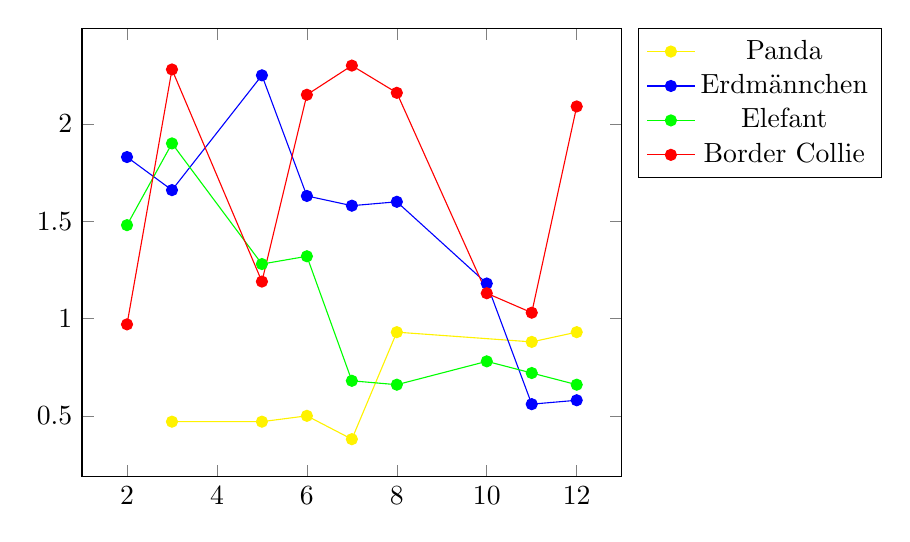
\begin{tikzpicture}
	
	\begin{axis}[legend pos=outer north east]
		\addplot[mark=*,yellow]
		coordinates {
			(3,.47) (5,.47) (6,.5) (7,.38) (8,0.93) (11,.88) (12,.93)
		};
		\addlegendentry{Panda}
		\addplot[mark=*,blue]
		coordinates {
			(2,1.83)(3,1.66)(5,2.25)(6,1.63)(7,1.58)(8,1.6)(10,1.18)(11,.56)(12,.58)
		};
		\addlegendentry{Erdmännchen}
		\addplot[mark=*,green]
		coordinates {
			(2,1.48)(3,1.9)(5,1.28)(6,1.32)(7,0.68)(8,0.66)(10,.78)(11,.72)(12,.66)
		};
		\addlegendentry{Elefant}
		\addplot[mark=*,red]
		coordinates {
			(2,.97)(3,2.28)(5,1.19)(6,2.15)(7,2.3)(8,2.16)(10,1.13)(11,1.03)(12,2.09)
		};
		\addlegendentry{Border Collie}
		
	\end{axis}
\end{tikzpicture}
\section{Computational Thinking Test}
	\subsection{Einordnung der Gruppe}
	
	\subsection{BCTt und CTt}